\documentclass[]{article}

\usepackage{amsmath}
\usepackage{listings}
\usepackage{clrscode}
\usepackage{algorithm}
\usepackage{algorithmic}
\usepackage{graphicx}
\usepackage[top=2cm, bottom=2cm, left=2cm, right=2cm]{geometry}

\title{Algorithm Homework 1}
\date{2015-10-8}
\author{Jingwei Zhang 201528013229095}

\begin{document}
    \maketitle
    \section{Problem 1}
        \subsection{Algorithm}
            \paragraph{} The problem given can be converted to a equivalent problem: Given two sorted array $A$ and $B$ with length $N$, find the $N$-th element $C[N]$ in the merged sorted array $C$ with length $2N$. Find a algorithm using $ O(\log n) $ queries for $ A[k] $ or $ B[k'] $.
            \paragraph{} The basic idea of my algorithm is dividing the array currently dealing with $A'$ and $B'$ with length $l$ into two parts $A'_l$(left part, smaller than $A'[\frac{l}{2}]$), parts $A'_r$(right part, larger than $A'[\frac{l}{2}]$) and $B'_l$, $B'_r$. By comparing $A'[\frac{l}{2}]$ and $B'[\frac{l}{2}]$, determining the possible part containing medium of the two array.
            \subparagraph{} For $A'[\frac{l}{2}] = B'[\frac{l}{2}]$, the medium is $A'[\frac{l}{2}]$ or $B'[\frac{l}{2}]$.
            If $A'[\frac{l}{2}] \leq B'[\frac{l}{2}]$, then $A'[i](i=0,\dots,\frac{l}{2}-1)$ must be located at $[0,l)$ of the merged array and $B'[i](i=\frac{l}{2}-1,\dots,\l-1)$ must be located at $[l+1,2l)$ of the merged array, which do not contain the medium. So the Problem become find the medium in $A'[\frac{l}{2},l)$ and $B'[0,\frac{l}{2}]$ . 
            For $A'[\frac{l}{2}] \geq B'[\frac{l}{2}]$, it is similar.
            
            \paragraph{Pseudocode:}
\begin{codebox}
\Procname{$\proc{Find-Medium}(A,B,l_A,r_A,l_B,r_B)$}
\zi    \Comment Find the medium number from $A[l_A,r_A)$ and $B[l_B,r_B)$
\zi    \Comment Index starts from 0
\zi    \Comment $A[k]$ means query the k-th smallest element in A
\li    \If $r_A - l_A == 1$
\li        \Then \Return $ min(A[l_a],B[l_a])$
       \End
\li    \If $r_A - l_A == 1$
\li        \Then Query for all 4 numbers$A[l_A],A[l_A+1],B[l_B],B[l_B+1]$
\li        $ans = $The second small number among these 4 numbers
\li        \Return ans
           \End
\li    $m_A = \lfloor \frac{l_A+r_A}{2} \rfloor$
\li    $m_B = \lceil \frac{l_B+r_B}{2} \rceil$
\li    \If $A[m_A]==B[m_B]$
\li        \Then \Return $A[m_A]$
\li    \ElseIf $A[m_A] \leq B[m_B]$
\li        \Then \Return $\proc{Find-Medium}(A,B,m_A,r_A,l_B,m_B+1)$
\li    \ElseNoIf \Return $\proc{Find-Medium}(A,B,l_A,m_A+1,l_B,r_B)$
       \End
\end{codebox}

        \subsection{Sub problem Reduction Graph}
            \paragraph{}See graph section.
        \subsection{Correctness}
            \paragraph{} As mentioned in algorithm part, the cutting operation guarantees that the medium is not in the cut part and one cut part smaller than the medium and one part greater than the medium. And the two part have the exactly the same length. So by cutting the two part, the medium of original array is the medium of the array left and the two arrays left have exactly the same length, which are maintained during the recursion.
            \paragraph{} When the length of each array is reduced to one the medium of these two is the smaller one. When the length of each array is reduced to two, one possible condition is that we will not cut it since one part has length 0 and then recursion will not end. So we list all numbers then pick 2nd. This guarantees recursion will stop.
        \subsection{Complexity}
            \paragraph{} We can make the length of array left  denote the size of this problem. During each recursion, we query for $A[m_A]$and$B[m_B]$, that is $O(1)$ and the total length is half of origin. So we can get:
            \begin{equation*}
                T(n) = T(n/2) + O(1)\\
            \end{equation*}
            
            \paragraph{} Since:
            \begin{align*}
                T(n) &= T(n/2) + O(1) \\
                     &= \sum_{1}^{\log{n}} {O(1)} \\
                     &= O(\log n)
            \end{align*}
            \paragraph{} So we will query for $O(\log n)$ totally.
    
    
    
    \section{Problem 3}
        \subsection{Algorithm}
            \paragraph{} The idea is almost the same as Merge and Count as long as we add one pointer pointing the possible inversions and count them. We count inversions of every number ing the right part, that  is from the first number greater than 3 times of this in the left part to the last number of left part.
            \paragraph{Pseudocode:}
\begin{codebox}
\Procname{$\proc{Sort-Count}(A)$}
\li    Divide A into two sub-sequence L and R
\li    $(RC_L,L) = \proc{Sort-Count}(L)$
\li    $(RC_R,R) = \proc{Sort-Count}(R)$
\li    $(C,A) = \proc{Merge-Count}(L,R)$
\li    \Return $(RC=RC_L+RC_R+C)$
\End

\end{codebox}
\begin{codebox}
\Procname{$\proc{Merge-Count}(L,R)$}
\li    $RC=0,i=0,j=0,p=0$
\li    \For $k=0$ \To $||L||+||R||-1$ 
\li        \Do                         \label{li:p_start}
\li            \While $L[p] < 3R[j]$
\li                \Do $p++$
               \End                    \label{li:p_end}
\li            \If $L[p] > R[j]$
\li                \Then $RC += (\frac{n}{2}-p)$ \label{li:count}
               \End
\li            \If $L[i] > R[j]$
\li                \Then $A[k] = R[j++]$
\li            \Else 
\li                $A[k] = L[i++]$
               \End
       \End
\end{codebox}
        \subsection{Sub problem Reduction Graph}
            \paragraph{}See graph section.
        \subsection{Correctness}
            \paragraph{} During reduction, we guarantee that the array dealing with is sorted and we have counted all inversions within this problem. The correctness of sorting is the same as merge sort so we will not cover that.
            \paragraph{} Suppose we have two sub arrays(L and R) sorted and counted all inversions within each array. Now, for merged array(A), it only contains the "cross" inversions between the left sorted part and right sorted part. The total cross inversions can be the sum of inversions contains each element of R.
            \paragraph{}When scanning element in R from left to right(current index j). L[p] is always the smallest element guaranteeing $L[p] > 3R[j]$(note that $L[p] \leq 3R[j]$). For the first element it is obvious, the while loop begins on line \ref{li:p_start} in MERGE-COUNT does that. So all elements right side $L[p]$(included) can from an inversion with $R[j]$. That is what line \ref{li:count} does. When j goes to j+1, note that $R[j] \leq R[j+1]$, so $L[p-1] \leq 3R[j] \leq 3R[j+1]$, so the smallest element $k$ guaranteeing $L[k] > 3R[j]$ is at least $p$. Then the While loop on line \ref{li:p_start} performs a linear search which guarantees $L[p'] > 3R[j+1]$ after that.
            \paragraph{}From all above, we have proven the correctness of this algorithm.
        \subsection{Complexity}
            \paragraph{} Dividing two sub problems costs only constant time. Problem is divided into two sub problems, each with half size.Since $i,j,k$ only grow, it costs liner time to combine two sub problems. So we can get:
            \begin{equation*}
                T(n) = 2T(n/2) + O(n)
            \end{equation*}
            \paragraph{} According to master theory:
            \begin{equation*}
                T(n) = O(n log n)
            \end{equation*}
            
            
            
    \section{Problem 6}
        \subsection{Algorithm}
            \paragraph{} For a given convex polygon,a specific edge may belong to different triangles. Such a triangle divide the polygon into two small polygons(it may degraded to one small polygon). Then when such a triangle exists, the number of total possible partitions will be the production of the numbers of possible partitions of these two small polygons. These small problems can be solved recursively since there is only one way for triangle. So we can enumerate all triangles containing this specific edge, compute all these number of partitions and then add them up.
            \paragraph{} To avoid computing the same problem repeatedly, we can store the result into an array A.
            \paragraph{Pseudocode:}
\begin{codebox}
\Procname{$\proc{Count-Partition}(n)$}
\zi    \Comment $A$ is the array storing results of smaller problems
\zi    \Comment Index denotes the size of problem(vertices of the convex polygon)
\li    \For $i = 0$\To $3$ 
\li        \Do $A[i] = 1$ \Comment Leting $A[0]$ to $A[2]$ equals $1$ can make multiplication simpler.
       \End
\li    \For $i = 4$\To $n$ 
\li        \Do $A[i] = -1$ \Comment Marked not computed yet.
       \End
\li    \Return \proc{Count-Formular}(n)   
\end{codebox}
\begin{codebox}
\Procname{$\proc{Count-Formular}(n)$}
\li    \If $A[n] > 0$ 
\li        \Then \Return $A[n]$
\li    \Else
\li        $sum = 0$
\li        \For $i = 1$ \To $n-2$
\li            \Do $sum+=A[i+1] * A[n-i]$ \label{Count-Formular:summing}
           \End
       \End
\li    \Return $sum$

\end{codebox}
        \subsection{Sub problem Reduction Graph}
            \paragraph{}See graph section.
        \subsection{Correctness}
        \begin{itemize}
            \item Firstly, the correctness of division. From geometry, we know that linking every two non-adjacent vertices will form two small convex polygon. So such a triangle will divide the big convex polygon into two small ones. 
            \item Then, the correctness of computing from small problems to big problem.
            \begin{itemize}
                \item Since one edge can below to $n-2$ different triangles and in every partition this edge must from a triangle with another vertex, total partition can be divided into $n-2$ types,these include all possible partitions.
                \item For partitions in different types, the dividing triangle is different, so they are different.
                \item For one type, the two small problems are independent, so we can simply multiply the number of these two.
            \end{itemize}
            So, combining small problems into big one include all situations non-repeatedly.
             
            \item Finally, obviously, for $n=3$ only one partition can be found.For $n=2$ let it equal $2$ to make it computable for multiplication.Thus the recursion will end.
        \end{itemize}
        \subsection{Complexity}
            \paragraph{}The size of this problem can be denoted by the number of vertices of convex polygon. Note for array $A$ every item was computed at most once and if we separate the summing up part and recursion part on line \ref{Count-Formular:summing}, which have no influence on the running time, when computing $A[k]$(summing up part), $A[i],i = 1,\dots,k-1$ has been computed. So if we analysis a "bottom-up" approach(actually it is the recall part of "top-down" approach), we can get:
            \begin{align*}
            T(n) &= T(n-1) + \sum_{1}^{n-2} {O(1)} \\
                 &= T(n-1) + O(n) \\
                 &= \sum_{i=3}^{n} {O(i)} \\
                 &= O(n^2)
            \end{align*}
            \paragraph{} So the time complexity is $O(n^2)$ and space complexity is $O(n)$, since we use a extra array A with length $n$.
        
    \section{Sub problem Graph}
        \begin{figure}[H]
			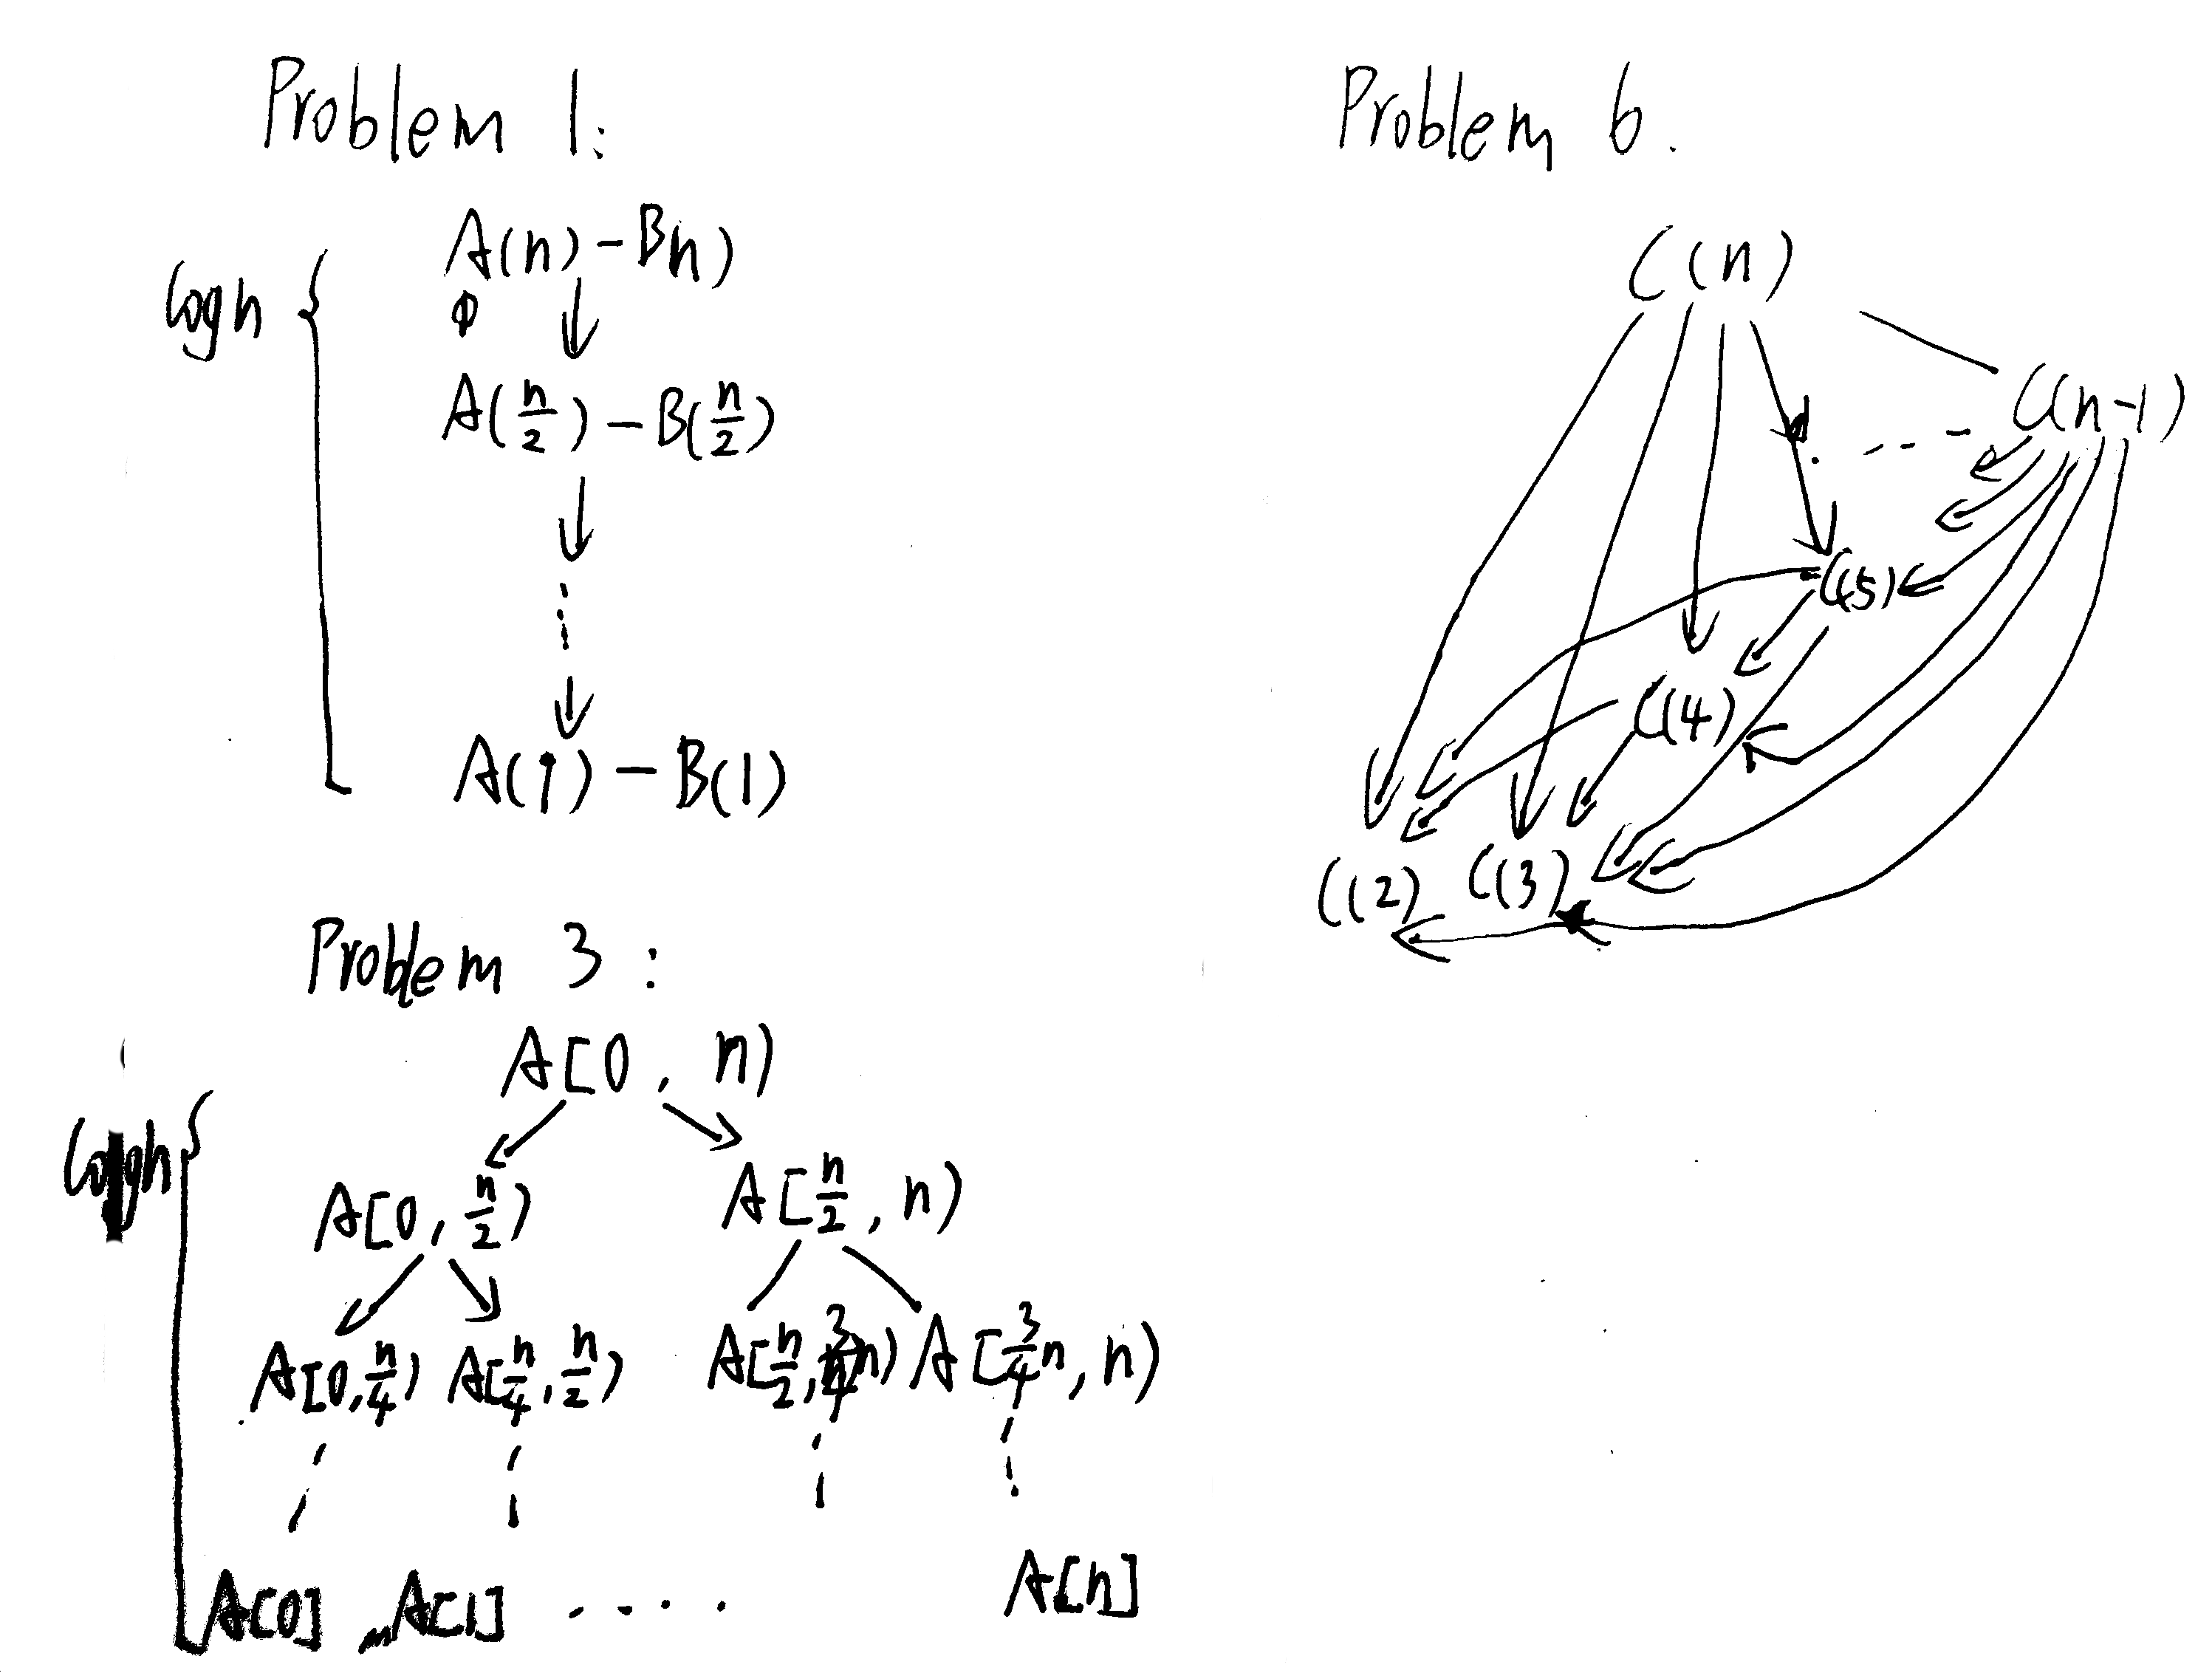
\includegraphics[scale=0.3]{sub_problem.png}
			\caption{subproblem reduction graph}
		\end{figure}

    
        
    \section{Problem 7}
        \subsection*{Method}
            \paragraph{}It is Possible to count inversions using quick sort algorithm in $ O(n \log n) $ time. We can count inversions during the partition. In every recursion:
            \begin{itemize}
                \item count the inversions between pivot and others,
                \item count "relative" inversions between left part(smaller than pivot) and right part(larger than pivot),
                \item guarantee the relative order of numbers in the left part is exact the same as the ralative order of these numbers in the original sequence, so does the right part.
            \end{itemize}
        \subsection*{Result}
            \paragraph{} Both report that there are 2500572073 inversions in given sequence.
            \paragraph{} Running time varies when program runs repeatedly, generally they are almost the same, around 12ms. It is hard to say which runs faster under such circumstance.
        \subsection*{Code}
        \lstinputlisting[language=C++]{Counting_inversions.cpp}
    \section{Problem 10}
        \subsection*{Result}
            \paragraph{} Below is a table showing the Runing time of Karatsuba Algorithm and grade school method.
            \begin{table}[h!]
            \centering
            \caption{Camparation: Running Time of Two algorimthss}
            
            \begin{tabular}{l|*{6}{r}}
            \hline
                Length N (Decimal)           & 1280 &
                    2560 & 5120 & 10240 & 20480 & 40960 \\
            \hline
                Grade School Method(ms)   & 21   & 
                    86 &   346  & 1389 & 5526   & 22047  \\
                Karatsuba Algorithm(ms)   & 86   & 
                    241 &  738  & 2192 & 7010   & 19952 \\
            \hline            
            \end{tabular}
            \end{table}
            \paragraph{} From table above we can see that grade school method runs faster when N is small, but when N grows, their difference gets smaller and finally when N = 40960 Karatsuba Algorithm wins.
        \subsection*{Code}
        \lstinputlisting[language=C++]{Karatsuba_Interger_Multiplication.cpp}
\end{document}